\documentclass[12pt, oneside]{report}
\usepackage[a4paper, width=160mm, height=245mm, top=15mm, bottom=22mm, left=30mm, right=20mm, head=3mm, foot=10mm]{geometry}
\usepackage{graphics}
\usepackage{graphicx}
\usepackage{amsmath}
\usepackage{float}
\usepackage{setspace}

\renewcommand{\baselinestretch}{1.5} 
\setlength{\parindent}{2.5cm}

\usepackage{fancyhdr}
\pagestyle{fancy}
\fancyfoot{}
\fancyfoot[CE, CO]{\thepage}
\fancyfoot[LE, LO]{Study of Gyrotron}
\fancyfoot[RE, RO]{Vaibhav Balloli}
\renewcommand{\headrulewidth}{0.5pt}
\renewcommand{\footrulewidth}{0.5pt}

\date{2018}

\pagenumbering{roman}
\setcounter{tocdepth}{4}

\begin{document}

\begin{titlepage}
	\thispagestyle{empty}
	\begin{center}
	\vspace*{1cm}
	
	\LARGE
	\textbf{Report Titled}
	
	\vspace{0.5cm}
	
	\Huge
	\textbf{Study of Gyrotron}
	
	\vspace{1.5cm}
	
	{\Large Submitted}\\
	{\Large in partial fulfillment of}\\
	{\Large the requirements of the degree of}\\
	[0.5cm]
	{\Large Bachelor of Engineering}\\
	{\Large (Electronics and Communication Engineering)}\\
	
	\vfill
	
	\Large
	By\\
	Vaibhav Balloli\\
	2016AAPS0165H\\
	\vspace{0.5cm}
	(2018)
	
	\vfill
	
	\Large
	Prof. Harish Vijay Dixit\\
	(Supervisor)
	
	\vfill
	
	\Large
	(Department of Electrical Engineering)\\
	(2018)
	
	
	\end{center}

\end{titlepage}

\chapter*{Abstract}
This report introduces gyrotron, a high power device, accounts for its brief history in the past century and its working principle. Later, the report describes various gyro-devices where the principle of gyrotron is used and compares their performance and concludes a suitable operation condition. Finally, the report ends with discussing about real-world applications of Gyrotrons.
\addcontentsline{toc}{chapter}{\numberline{}Abstract}

\cleardoublepage

\tableofcontents

\listoftables
\thispagestyle{empty}

\listoffigures
\thispagestyle{empty}

\pagenumbering{arabic}
\chapter{Introduction}
\setcounter{page}{1}
\thispagestyle{empty}
Gyrotrons are high-power devices based on vacuum tubes that produce millimeter-wave electromagnetic waves. Their operating principle is based on Electron Cyclotron Resonance, a phenomenon where stimulated cyclotron radiation of electrons oscillating in a strong magnetic field transfer their energy to the field. These devices operate in the frequency range 10 - 95 GHz and researchers are still trying to find ways to expand this range to terahertz(THz). Gyrotrons can provide power from 10kW to 2MW and can be used in both continuous wave and short-pulse modes.\\

Gyrotrons are termed as fast-wave devices because the size of the interaction structure of these devices exceed the wavelength of the radiation generated unlike slow-wave devices, whose interaction structures are of the order of the wavelength of the waves generated, by them.\\

Gyrotrons are capable of generating high power without causing much damage to the structure due to the large amount of heat produced because the interaction cavity inside the gyrotrons are made of copper making them easier to maintain and reduce their temperature.

\chapter{History}
\section{Prehistory}\label{sec:beginning}
The prehistory of the basic concept of working of gyrotron dates to the twentieth century where scientists tried to generate electromagnetic waves by radiation of oscillating electrons .Theoretically, the research on this phenomenon was started by 
Gaponov and Pental in the 1959 based on the research in Electron Cyclotron Resonance by Twiss in Australia, Schneider in the USA and Gaponov in the USSR, whose results were then published by scientists of USA and USSR.\cite{ref:tg}\cite{ref:gt}
 
A gyrotron was constructed at the Tadio-Physical Institute, Gorki, USSR in 1963 consisting of:

\begin{enumerate}
\item Annular Magnetron electron gun
\item Adiabatic Compressor for the rotating stream of electrons
\item Smooth walled cavity
\end{enumerate}

The first working gyrotron was constructed by Hirshfield and Wachtel in 1964. This gyrotron supplied 6W of power at 10GHz frequency in the CW mode. MIG (Magnetron Injection Gun) replaced the annular magnetron gun along with a single cavity which resulted in higher efficiency and increased power output.

\section{Development}
The progress in the development of the gyrotron gained in 1980s, both in the theoretical and experimental aspects including other devices based on the same principle like gyro-TWT, gyro-klystron  etc. This era of development primarily dealt with elimination of parasitic oscillation, proper profiling of the cavity, increasing the work frequency and the development of tunable gyrotrons. This led to inclusion of helical output launcher developed by Vlasow in the same period. Many countries like France, Korea, Germany, Australia also joined the research, building their own gyrotrons later during the 1980s.

\section{Current Stage}
 Recently, China and India started researching and developing their own gyrotrons due to which a drastic improvement occurred in the development of tetrahertz and co-axial gyrotrons. The most significant contribution to the current state of gyrotrons is by ITER (International Thermonuclear Experimental Reactor), an international nuclear fusion research and engineering project led by seven entities - European Union, India, Japan, China, Russia, South Korea, and the United States to build the world's largest magnetic plasma confinement experiment.


\chapter{Principle of Working}
Gyrotron is based on the phenomenon termed as ECR (Electron Cyclotron Resonance) which is instability caused to relativistic rotating electrons in a constant magnetic field, with an electric field of the electromagnetic wave which causes electrons to oscillate and radiate electromagentic waves, hence classifying this device as a CEM (Classical Electron Maser).\\

A free electron moves along a toroidal trajectory when subject to a uniform static electric and magnetic field. The electron gun in the gyrotron generates a hollow beam of electrons, consisting of smaller beams called beamlets. Each electron in every helical beamlet is subjected to an alternating electric field.\\

\begin{figure}
\centering
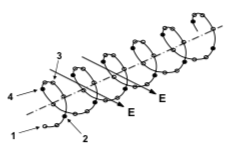
\includegraphics{./images/beamlet}
\caption{A beamlet travelling along the tube in the electric field}
\label{fig:beamlet}
\end{figure}

Considering one beamlet ( see figure \ref{ fig:beamlet } ), the electrons in position number 1 and 3 along the helical beam encounter deceleration and acceleration respectively, as each of them are moving in the direction and opposite to the direction of  electric field at that instant respectively. Electrons in positions 2 and 4 are moving perpendicular to the field so their mass is not being affected. This varying effect of electric field on various positions on the helix causes the electrons to form bunched electrons moving along the direction of electric field, energy is lost by the electron bunch indicating transfer of energy from the electrons to the electric field on each half-cycle of the alternating field.\\

The combination of many beamlets undergoing loss of energy every half-cycle causes amplification of the field when all of them synchronize.
\chapter{Gyro-devices}
Since gyrotrons are ECMs, the gyro-devices are classified according to their functionality and dispersion diagrams, that are designs based on the concept of wave-particle interaction. Dispersion diagrams, also called w-kz plots or Brillouin diagrams, show the region of cyclotron interaction (maximum gain of the instability) between an electromagnetic mode and a fast electron cyclotron mode (fundamental or harmonic) as an intersection of the waveguide mode dispersion curve (hyperbola): $ w2 = k z^2 c^2 + k'^2 c^2 $

\section{Gyro-oscillators}
Gyro-oscillators are capable of providing high power in pulse mode or low power in CW (Continuous Wave) modes.  These gyrotrons are now being used in short and long pulse Megawatt-class gyrotrons.
\subsection{Gyro-monotron}
Gyro-monotrons are generally referred as gyrotrons. These devices are a type of ECR (Electron Cyclotron Maser) that underwent major development.  In 1964, IAP Nizhny Novgorod built and operated the first gyrotron in TE101 mode producing 6W power in CW mode. The device's output power increased when the originally used electron gun was replaced by Magnetron Injection Gun in tapered, open-ended waveguide cavities that maximize efficiency by tailoring the electric field distribution in the resonator. These devices are operated at resonant frequencies (see figure \ref{fig:gmd} ) Sometimes, the gyrotron can be operated at higher harmonics with lower fundamental frequencies and efficiencies.

\subsection{Gyro-BWO}
Gyro-BWO(Back Ward Oscillators) are similar to gyro-monotrons except for the wave interaction where the electron beam and/or magnetic field is adjusted so that the straight fast-wave beam line crosses the negative kz-branch of the waveguide mode (see figure \ref{fig:gbd} ) creating instability due to the formation of a backward-wave (internal feedback). These devices are used to generate moderately high power, but work at relatively lower frequencies and efiiciencies compared to the standard gyrotron.\cite{ref:bwo}

\begin{figure}[H]
\centering
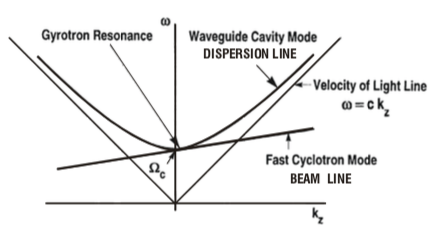
\includegraphics[scale=0.8]{images/gyro_mono_dispersion}
\label{fig:gmd}
\caption{Dispersion diagram of Gyro-monotron}
\end{figure}
\begin{figure}
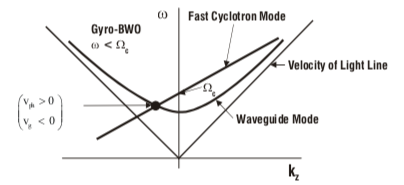
\includegraphics{images/gyro_bwo_dispersion}
\label{fig:gbd}
\caption{Dispersion diagram of Gyro-BWO.}
\end{figure}



\subsection{Performance}
The following tables contain data of short-pulsed gyrotron and relativistic pulse gyro-BWOs (tables \ref{tab:spgm} and \ref{tab:spgb} ).

\begin{table}[H]
	\begin{tabular}{c|c|c|c|c}
	Institution & Frequency (GHz) & Cavity Mode & Power (MW) & Efficiency (\%) \\
	\hline
	CPI/MIT/GA & 110 & TE22,6 cylindrical & 1.5 & 48 (SDC)\\
	FZK/EFDA & 165 &TE31,12 coaxial & 2.2 & 48 (SDC)\\
	GYCOM/IAP & 170 & TE28,12 cylindrical &1.44 & 41 (SDC)\\
	TED/EFDA & 170 & TE34,19 coaxial & 1.8 & 28\\
	Toshiba/JAEA & 170 & TE31,12 cylindrical & 1.56 & 27
	\end{tabular}
	\caption{Short-Pulse 1.5–2 MW Gyro-monotrons\cite{ref:soa} }
	\label{tab:spgm}
\end{table}

\begin{table}[H]
	\begin{tabular}{c|c|c|c|c}	
	Institution & Frequency (GHz) & Cavity Mode & Power (kW) & Efficiency (\%) \\
	\hline
	IAP, N. Novgorod & 24.7 & TE1,1 & 7 & 7\\
	UNIV. Hsinchu & 33.5 & TE1,1 & 40 & 15
	\end{tabular}
	\caption{Relativistic Short-Pulse Gyro-BWO\cite{ref:soa} }
	\label{tab:spgb}
\end{table}

The above metrics\cite{ref:soa} indicate that:
\begin{enumerate}
\item The standard gyrotron/gyro-monotron devices are capable of operating at very high frequencies (100+GHz) and are capable of giving an output power of 1-2 MW.
\item The gyro-BWO operate at relatively lower frequency and output lower power.
\item

Each of the gyro-oscillators have clear applications according to the requirements, but most applications use the standard gyrotron oscillators to exploit the property of generating high power.
\end{enumerate}


\section{Gyro-Amplifiers}
The devices that come under gyro-amplifiers are :
\begin{enumerate}
\item  Gyro-klystron
\item  Gyro-twystron
\item Gyro-TWT
\end{enumerate}

Gyro-amplifiers are being developed and deployed to fields where there's a need for coherence and instantaneous bandwidth. Gyro-amplifiers are huge in terms of weight and volume than state-of-the-art coupled- cavity TWT, but provide significantly higher power than the TWTs. The wide variety of radar applications for which gyro-amplifiers are now being considered, which wasn't the case earlier due to the absence of powerful amplifiers at the required frequencies. The bandwidth requirement of the application determines the tube type:

\begin{enumerate}
\item Gyro-klystron for less than 1\% bandwidth
\item Gyro-twystron for 1\% to 2\% bandwidth
\item Gyro-TWT for bandwidths greater than 2\%
\end{enumerate}

\subsection{Gyro-Klystrons}
Conceptually, gyro-klystrons are gyrotron oscillators with an additional input cavity added to the structure ( see figure \ref{fig:gky} ). The operation of a gyro-klystron is similar to a conventional klystron except that electron bunching (gyro) occurs in the azimuthal than in axial direction. In a gyro-klystron,  the input signal is fed into input cavity, the new addition to the gyro-oscillator where the cyclotron bunching process is initiated. Then, the beam passes through the tube as bunches form. As the beam passes through a second cavity, the amplified signal may be removed or the bunching process may be enhanced and the signal is then removed in the subsequent cavity.

\begin{figure}[H]
\centering
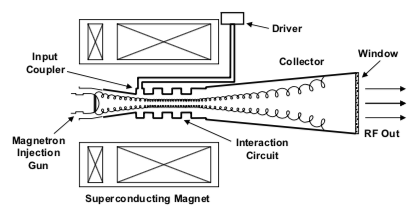
\includegraphics[scale=0.8]{images/gyro_klystron}
\label{fig:gky}
\caption{Gyro-klystron}
\end{figure}

\subsection{Gyro-Twystron}
The gyro-twystron is very similar to a conventional twystron, which is a hybrid device with a moderate bandwidth. The structure is derived from the gyro-klystron by using gyro-klystron's interaction in the cavities near the RF input and replacing it's output cavity with a slightly tapered waveguide section as in a gyro-TWT. The output section is excited by the electron beam, which is bunched by the interaction in the klystron section. This structure of the gyro-twystron doesn't suffer with the problem of having a breakdown at high-power levels because the radio frequency power density in the output waveguide is smaller than in the gyro-klystron output cavity.

\subsection{Gyro-TWT}
Of all the gyro-amplifiers, the gyro-TWT has gathered the a lot interest and is actively researched. In millimetre-wave radars, the gyro-TWT is a proper fit as the transmitter power amplifier. Gyro-TWTs are capable of operating at broader bandwidths than gyro-klystrons. In gyro-TWTs, a non-resonant RF structure is used to produce a traveling wave interaction, unlike other gyro-devices, where a spiraling electron beam immersed in an axial magnetic field is used. In this device, Traveling waves are launched into the interaction space by an input coupler. As the spiraling electron beam moves through the interaction space along with the electromagnetic wave, it loses energy to the electromagnetic field i.e it is transferred into the electromagnetic fields, creating an RF amplification. In a usual operation, the device is operated near the cutoff frequency of the interaction waveguide, where the transverse component of electron motion interacts with the electromagnetic wave (in the same direction) .

Most of the interaction space exhibits a moderate amount of electromagnetic loss per unit length to ensure stability of the device. This distributed loading approach has been shown to have superior stability characteristics. Finally, the downstream part of the interaction space is completed with a short, unloaded cylindrical tunnel in which the final, highest powered portion of the amplification takes place.

\subsection{Performance}
The following tables comprises data of relativistic short-pulsed gyro-klystron,  short-pulse gyro-twystrons and short-pulse gyro-TWTs (tables \ref{tab:spgk}, \ref{tab:spgt}, \ref{tab:spgtw} ).

\begin{table}[H]
	\resizebox{\columnwidth}{!}{
	\begin{tabular}{c|c|c|c|c|c|c}	
	Institution & Frequency (GHz) & Cavity Mode & No. of Cavities & Power (MW) & Efficiency (\%) & Bandwidth(\%) \\
	\hline
	UNIV. Maryland & 8.57 & TE0,1 & 3 & 75 & 32 & 0.2\\
	IAP, Nizhny Novgorod & 30 & TE5,3 & 2 & 5 & 25 & 0.14
	\end{tabular}}
	\caption{Relativistic Short-Pulse Gyro-Klystrons\cite{ref:soa} }
	\label{tab:spgk}
\end{table}

\begin{table}[H]
	\resizebox{\columnwidth}{!}{
	\begin{tabular}{c|c|c|c|c|c|c}
	Institution & Frequency (GHz) & Cavity Mode & No. of Cavities & Power (MW) & Efficiency (\%) & Bandwidth(\%) \\
	\hline
	UNIV. Maryland & 9.87 & TE0,1 & 2 & 21.6 & 21 & 1-2\\
	UNIV. Maryland & 19.76 & TE0,1 & 2 & 12 & 11 & 1-2
	\end{tabular}}
	\caption{Relativistic Short-Pulse Gyro-Twystrons\cite{ref:soa} }
	\label{tab:spgt}
\end{table}

\begin{table}[H]
	\resizebox{\columnwidth}{!}{
	\begin{tabular}{c|c|c|c|c|c|c}
	Institution & Frequency (GHz) & Cavity Mode & No. of Cavities & Power (MW) & Efficiency (\%) & Bandwidth(\%) \\
	\hline
	IAP, Nizhny Novgorod & 79.4 & TE1,1 & & 1.1 & 29 & 2.1\\
	NRI, Washington D.C & 35 & TE1,1 & &20 & 11 & NA
	\end{tabular}}
	\caption{Relativistic Short-Pulse Gyro-TWTs\cite{ref:soa} }
	\label{tab:spgtw}
\end{table}

The above metrics\cite{ref:soa} indicate that (as mentioned in the introduction of gyro-amplifiers) each of these devices have applications based on the required bandwidth and operating frequency.
\begin{enumerate}
\item Gyro-klystrons are the most efficient gyro-amplifiers operating at relatively low frequencies and bandwidth.
\item Gyro-twystrons, compared to the other two amplifiers, operates at lower frequency with lower efficiency, the only advantage being the operation bandwidth.
\item Gyro-TWTs are efficient devices capable of operating at higher frequencies and higher bandwidth.

Gyro-TWTs and gyro-klystrons are clear choices for applications requiring high output power like radars, where these devices are now being used.

\end{enumerate}

\chapter{Applications}
Gyrotron has many applications spanning across a variety of fields due to its capability of generating high power at high frequencies.
Some of these fields include spectroscopy, plasma heating and diagnosis, defence that indicate applicability of gyrotrons.

\section{Defence}

National security is always a top priority for all countries and this leads to development of cutting edge instruments and devices that can help detect all kinds of threats, from a unknown drone to space junk near space stations and act accordingly, to protect their citizens and interests.

\subsection{Military}

Raytheon of the U.S. Army used gyrotrons, gyro-amplifiers in a system they developed, called the Active Denial System (ADS). The ADS system ( see figure \ref{fig:ads} ) is a non-lethal, anti-personnel weapon that uses the directed energy of the gyrotron. The gyrotron used works at 95GHz with an effective power density of $ 2W/m^2 $ covering 1km radius. This device generates waves that penetrates the skin causing a spike in water's temperature thus heating the upper layer of the skin upto 60 degrees celsius causing a second degree burn and inflicting serious pain.

\begin{figure}[H]
\centering
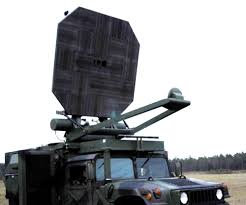
\includegraphics{images/ads}
\caption{Active Denial System, U.S.Army.}
\label{fig:ads}
\end{figure}

\subsection{Radar}

Current radar technologies are based on millimetre wave radars that can fetch high location resolution of tracked objects. Using gyro-sources, primarily the gyro-amplifier gyro-TWT and gyro-klystrons, the effective range of these radars has risen upto several hundred kilometres, which combined with high resolution imaging, gives best results. Russia and U.S.A are using gyro-klystrons based antennas, providing output power in the range of 0.1-0.5 MW.

\section{Scientific Research}

Science has had a need for high power and high frequency devices from the past two centuries and the gyrotrons have shown some good prospects and development in some particular fields. Here, gyrotrons are used as gyrotron oscillators.

\subsection{Nuclear Fission and Plasma}
Nuclear fission and plasma research have extensively focussed on developing gyrotrons which have played a huge role in the progress of the field. ITER (International Thermonuclear Experimental Reactor). The ITER required a highly efficient device capable of generating high output power and long pulse of generated radiation to carry out a controlled nuclear fusion. The ITER uses gyrotron at 170GHz generating output power of 1-2 MW.

\subsection{Material Science}
The radiations generated by gyrotrons are used by a technique called Electron Spin Resonance (ESR). Using this technique, the microstructures of various materials are investigated, studied and tested with the help of tetrahertz radiation. The tetrahertz radiation is also used along with Nuclear Magnetic Resonance (NMR). This NMR spectroscopy is used to study materials such as polymers and in bio-molecular analysis of protein and peptide structures that use low-power gyrotrons such as gyro-BWO to provide tetrahertz radiation.



\chapter{Results}
The performance data mentioned in previous sections clearly indicate the evolution and advancement in the metrics of gyrotrons over the past 50 years, Although gyro-amplifiers have greater advantage over gyro-oscillators, all these devices are still being deployed and used in many areas of science, based on requirement. Since these devices are capable of generating a huge amount of power, they come with additional liability of misusing them in lethal weapons, something already witnessed with magnetrons in the history of wars.
\chapter{Conclusions}
Gyrotrons are promising, useful devices that find it's applications in many fields, from plasma research to military technology. These devices have evolved a long way from being used as oscillators to amplifiers in cutting edge research. Further research into these devices is being conducted to operate at terahertz(THz) giving an output power in multiples of megawatt(MW) from the performance metrics of various research conducted at different institutions and companies.
\bibliographystyle{IEEEtran}
\bibliography{/Users/balli/Documents/emfme/references.bib}
\pagebreak
\thispagestyle{empty}
\begin{center}
\vfill
\textbf{\Large{Declaration of the Student}}
\end{center}
\vfill

\large {I declare that this written submission represents my ideas in my own words and where
others' ideas or words have been included, I have adequately cited and referenced the
original sources.\\

I also declare that I have adhered to all principles of academic honesty and integrity and
have not misrepresented or fabricated or falsified any idea / data / fact / source in my
submission.\\

I understand that any violation of the above will be cause for disciplinary action by the
Institute and can also evoke penal action from the sources which have thus not been
properly cited or from whom proper permission has not been taken when needed.\\
}

\vfill

\begin{flushleft}
\large{
	Vaibhav Balloli\\
	[0.2cm]
	2016AAPS0165H\\
	[0.2cm]
	Date: 02/11/18.
}
\end{flushleft}

\end{document}